% The frames of the results deck, shared by SLIDES_v7_2026-09-09.tex (plain) and
% SLIDES_v7_2026-09-09_annotated.tex (each slide followed by its notes). \slidenote{...}
% is defined by the wrapper: empty in the plain deck, a notes frame in the annotated one.
% Citations: [DFS21] Dick and Fernandez-Serra 2021 and the other keys of the last slide;
% [code: file:line] the repository line that implements the equation.

\begin{frame}
  \titlepage
\end{frame}
\slidenote{The deck condenses the full report (REPORT\_v7\_2026-09-09) and its summary. Six sections follow the pipeline: the model (Sec. 1), the generation of the training subsets (Sec. 2, the step before any network is fitted), the pre-training of each architecture to reproduce its parent functional (Sec. 3), the optimization on the training subsets read on the training data itself (Sec. 4), the held-out generalization (Sec. 5) and the pending work (Sec. 6). Bracketed keys cite the paper or the repository line an equation or value comes from; the keys are expanded on the last slide.}

\begin{frame}{Scope}
  One network pair (exchange and correlation) per architecture and training-subset size, as separate cluster runs under one protocol, drawn once over every finished cell (the runs merged into one view). Each run carries a pre-training (the cloning of the parent), a fidelity certificate that gates its training array, and the array itself, one cell per (architecture, subset size).
  \vspace{0.4em}
  \begin{center}\scriptsize
  \begin{tabular}{p{1.9cm}p{5.7cm}p{3.5cm}p{2.6cm}}
  \toprule
  Run & Architectures & Cells done / planned & Run directory \\ \midrule
  size & deep\_3x16, deep\_attn\_3x16 & deep\_3x16 11/11, deep\_attn\_3x16 9/11 & \path{run_20260902T145245Z} \\
  families & deep0\_3x16, deep0\_attn\_3x16, deep0\_cusp\_3x16 & deep0\_3x16 11/11, deep0\_attn\_3x16 2/11, deep0\_cusp\_3x16 0/11 & \path{run_20260902T145247Z} \\
  meta-GGA families & deep0\_cusp\_mgga\_3x16, deep0\_mgga\_3x16, deep0\_mgga\_attn\_3x16, deep0\_rung35\_mgga\_3x16, deep0\_rung35ms\_mgga\_3x16 & 0/55 (first certificate FAIL, four pending) & \path{run_20260902T145250Z} \\
  \bottomrule
  \end{tabular}
  \end{center}
  \vspace{0.3em}
  \begin{itemize}
    \item Subset sizes 1, 2, 3, 4, 5, 6, 7, 12, 15, 18, 26 points of the 26-point DFS pool [DFS21, SI Sec. II], chosen by Jensen-Shannon selection (Sec. 2).
    \item Basis 6-311++G(3df,2pd), grid level 3, density fitting, at every stage [cfg]. The validation-best checkpoint is read for every optimization figure.
  \end{itemize}
\end{frame}
\slidenote{\textbf{Cell:} one trained functional, identified by its architecture and the size of the training subset it was trained on; the size run has 44 cells of which 20 are finished, the families run 33 of which 13; every figure and table is drawn once over all 33 finished cells (the runs merged into one view). \textbf{Run:} a cluster run with one configuration file; the runs differ only in which architectures they train. \textbf{Pre-training:} fitting the networks to reproduce an existing functional (PBE or SCAN) before any training on reference data. \textbf{Fidelity certificate:} the check that the pre-trained networks reproduce the parent's energies to tolerance; if it fails, the group's training does not start. \textbf{Training array:} the cluster job array of cells. \textbf{DFS pool:} the training set of Dick and Fernandez-Serra's 2021 Letter. \textbf{Validation-best checkpoint:} training saves three checkpoints (final, lowest training loss, lowest validation error); the figures use the one with the lowest validation reaction-energy error. The basis, grid and density-fitting settings are those of the run configuration files (\texttt{dfs\_step7.dfs6311\_grid3\_v7*.yaml}) and are recorded in every certificate file.}

% =====================================================================
\section{1. Model}

\begin{frame}{1. Model: density variables and the DFS coordinates}
  With $n = n_\alpha + n_\beta$ and $\sigma = |\nabla n|^2$ [DFS21 Eqs. 4, 5]:
  \[
  k_F = (3\pi^2 n)^{1/3}, \qquad
  s = \frac{|\nabla n|}{2 k_F n}, \qquad
  r_s = \left(\frac{3}{4\pi n}\right)^{1/3},
  \]
  \[
  \zeta = \frac{n_\alpha - n_\beta}{n}, \qquad
  \phi(\zeta) = \tfrac12\left[(1+\zeta)^{4/3} + (1-\zeta)^{4/3}\right].
  \]
  The networks read logarithmic compressions of these [DFS21 Eqs. 7 to 10; code: networks.py:621--657]:
  \[
  x_0 = \ln\!\left(n^{1/3} + 10^{-5}\right), \qquad
  x_1 = \ln \phi(\zeta), \qquad
  x_s = \left(1 - e^{-s^2}\right)\ln(s + 1), \qquad
  x_\alpha = \ln\frac{\alpha + 1}{2}.
  \]
  \begin{itemize}
    \item Exchange input $[x_s, \ldots]$ with $s$ of the doubled spin channel $2 n_\sigma$ (the exchange network is evaluated per spin channel, next slides); correlation input $[x_0, x_1, x_s, \ldots]$ on the total density. The ellipsis holds the architecture's extra descriptors; on the meta-GGA rung the raw $\alpha$ is replaced by $x_\alpha$.
    \item The $10^{-5}$ in $x_0$ is the DFS reference implementation's constant [dpyscf net.py:39; code: networks.py:27].
  \end{itemize}
\end{frame}
\slidenote{$n$ is the electron density, $\sigma$ the squared gradient. $k_F$ is the Fermi wave vector of a uniform gas at density $n$; $s$ the reduced (dimensionless) density gradient, the GGA variable; $r_s$ the Wigner-Seitz radius (large where the density is low); $\zeta$ the spin polarization ($0$ closed shell, $\pm 1$ fully polarized); $\phi$ the spin-scaling factor that enters PBE correlation. The coordinates $x_0, x_1, x_s, x_\alpha$ are what the neural networks actually receive: logarithms compress the range of $n^{1/3}$ (which spans many orders of magnitude on a molecular grid) and of $s$, so that the network's inputs are of order one everywhere. $x_s$ behaves as $s^2 \ln(s+1)$ near $s = 0$ and as $\ln s$ at large $s$. The exchange network sees each spin channel separately at twice its density, which is how the exact spin-scaling relation of exchange is built in (next slides); the correlation network sees the total density and the polarization through $x_1$. The density is floored at a small cutoff before any of these variables is formed, so that the vanishing-density tail of the grid produces no infinities.}

\begin{frame}{1. Model: the extra descriptors}
  \textbf{Iso-orbital indicator} (meta-GGA rung; SCAN's $\alpha$ [SCAN15 Eq. 2; DFS21 Eq. 6; code: metagga.py:8--9]), a contraction of the live density matrix $P$ against the AO gradients, hence self-consistent and differentiable through the SCF:
  \[
  \alpha = \frac{\tau - \tau_W}{\tau_{\rm unif}}, \qquad
  \tau = \tfrac12 \sum_i |\nabla\psi_i|^2 = \tfrac12 \sum_{\mu\nu} P_{\mu\nu}\, \nabla\chi_\mu\cdot\nabla\chi_\nu,
  \]
  \[
  \tau_W = \frac{|\nabla n|^2}{8n}, \qquad
  \tau_{\rm unif} = \tfrac{3}{10}(3\pi^2)^{2/3} n^{5/3},
  \]
  with $\alpha \ge 0$ imposed by a smooth positive part rather than a hard clip [code: metagga.py:25--31].
  \vspace{0.4em}

  \textbf{Nuclear cusp pair} (\texttt{cusp}), two bounded geometric features per grid point [code: descriptors.py:230--245]:
  \[
  x_4 = \exp(-2 Z_{\rm nearest}\, r_{\min}), \qquad
  x_5 = \tanh\!\left(\frac{1}{5}\ln \sum_A \frac{Z_A}{r_A}\right),
  \]
  $x_4$ the density-form cusp envelope $e^{-2Zr}$ [Steiner63, after Kato57], $x_5$ the log-compressed bare-nuclear potential. Both are geometric, so the synthetic pre-training mesh (Sec. 3) carries no values for them.
\end{frame}
\slidenote{$\tau$ is the (positive) kinetic-energy density of the occupied orbitals $\psi_i$; on a basis set it is a contraction of the one-particle density matrix $P$ with the gradients of the atomic-orbital functions $\chi_\mu$, which is why it can be differentiated through the self-consistent field: it depends on the live density matrix, not on a frozen reference. $\tau_W$ is the von Weizsacker kinetic-energy density, the value of $\tau$ for a single occupied orbital, and $\tau_{\rm unif}$ the value for a uniform gas at the same density. $\alpha$ therefore reads 0 in a single-orbital (one-electron or covalent bond) region, 1 in a uniform-gas-like region, and grows in regions of overlapping closed shells. The lower bound $\alpha \ge 0$ holds exactly for a single occupied orbital but can be violated numerically; a smooth positive part keeps the derivative continuous there, which a hard clip would not. The cusp pair encodes where the nuclei are: $x_4$ is 1 at a nucleus and decays with the density's own cusp envelope (the electron density falls as $e^{-2Zr}$ near a nucleus of charge $Z$, the density counterpart of Kato's wavefunction cusp condition), $x_5$ is a bounded, log-compressed version of the bare nuclear potential summed over all nuclei. Because both depend only on the geometry, the synthetic $(r_s, s, \alpha)$ mesh used to regularize pre-training has no value to give them.}

\begin{frame}{1. Model: the functional form}
  \small
  MLP output $g$ at a grid point (GELU, \texttt{depth} $\times$ \texttt{nodes}) [code: networks.py:169, 379--404]:
  \[
  F_x = 1 + \mathcal{L}_{1.804}\!\left(G_x \cdot g_x\right), \qquad
  F_c = 1 + \mathcal{L}_{2}\!\left(G_c \cdot g_c\right),
  \]
  \[
  \mathcal{L}_{\lambda}(z) = \lambda\,\mathrm{sigmoid}\!\left(z - \ln(\lambda - 1)\right) - 1 \quad \text{[DFS21 Eq. 11]},
  \]
  \[
  G = \tanh^2(s) \ \ \text{(GGA)}, \qquad G = x_s + \tanh^2(x_\alpha) \ \ \text{(meta-GGA) [DFS21 Eq. 12]}.
  \]
  $\mathcal{L}_\lambda(0) = 0$ and $F \in (0, \lambda)$; $\lambda = 1.804 = 1 + \kappa_{\rm PBE}$ for exchange [PBE96 Eq. 14] (DFS uses 1.174 [PRSB14]), $\lambda = 2$ so that $F_c \ge 0$ [DFS21 Eq. 13]. The gate $G$ pins $F = 1$ where the gradient vanishes.
  \[
  E_{xc} = \tfrac12\left(E_x[2 n_\alpha] + E_x[2 n_\beta]\right) + E_c[n_\alpha, n_\beta] \ \ \text{[OP79; code: descriptors.py:124]},
  \]
  \[
  E_x[n] = \int n\, \epsilon_x^{\rm LDA}(n)\, F_x\, d^3r, \qquad
  E_c = \int n\, \epsilon_c^{\rm PW92}(r_s, \zeta)\, F_c\, d^3r \ \ \text{[PW92]}.
  \]
  \textbf{Attention variants} (\texttt{\_attn}) [Vas17 Eq. 1; Xio20; code: net.py:55--136]: after the first hidden layer, the $H$ hidden units are $h$ tokens of dimension $d_k = H/h$ under pre-layer-norm self-attention across the token axis, a per-point re-mixing of hidden units:
  \[
  \mathrm{Attn}(Q, K, V) = \mathrm{softmax}\!\left(\frac{QK^{\top}}{\sqrt{d_k}}\right) V, \qquad
  x \leftarrow x + W^{O}\,\mathrm{Concat}(\mathrm{head}_1, \ldots, \mathrm{head}_h)(\mathrm{LN}(x)).
  \]
\end{frame}
\slidenote{The functional is written as the local density approximation times an enhancement factor: $E_x = \int n\,\epsilon_x^{\rm LDA}(n) F_x$ for exchange and the same with the PW92 uniform-gas correlation energy per particle for correlation. $F_x = F_c = 1$ is the LDA; PBE, SCAN and the trained networks differ in how $F$ depends on the density variables. The network's raw output $g$ is passed through the bounded map $\mathcal{L}_\lambda$, which sends 0 to 0 and confines $F$ to $(0, \lambda)$; for exchange $\lambda = 1.804$ is the PBE ceiling derived from the Lieb-Oxford bound, for correlation $\lambda = 2$ merely guarantees $F_c \ge 0$ (the upper value is not used). The gate $G$ multiplies the network output by $\tanh^2(s)$, which vanishes where the gradient vanishes, so the uniform electron gas limit $F = 1$ is exact by construction; on the meta-GGA rung the DFS gate adds a term in $x_\alpha$. The exchange energy is assembled from the exact spin-scaling relation of Oliver and Perdew: exchange of a spin-polarized system is the average of the spin-unpolarized functional evaluated at twice each spin density; this is why the exchange network is evaluated per spin channel. The attention variants insert one self-attention block after the first hidden layer: the hidden vector at a grid point is cut into $h$ tokens, each token attends to the others with the standard scaled dot-product formula, and the result is added back (a residual) after a layer normalization. It re-mixes hidden units at one grid point; it does not look at neighbouring points, so the functional stays semilocal.}

\begin{frame}{1. Model: the architectures}
  \begin{center}\scriptsize
  \begin{tabular}{lllllll}
  \toprule
  Architecture & Last layer & Rung, parent & Hidden & Heads & Extra \\ \midrule
  deep\_3x16 & Glorot & GGA, PBE & 3 x 16 & none & none \\
  deep\_attn\_3x16 & Glorot & GGA, PBE & 3 x 16 & 4 & none \\
  deep0\_3x16 & zeroed & GGA, PBE & 3 x 16 & none & none \\
  deep0\_attn\_3x16 & zeroed & GGA, PBE & 3 x 16 & 4 & none \\
  deep0\_cusp\_3x16 & zeroed & GGA, PBE & 3 x 16 & none & cusp \\
  deep0\_cusp\_mgga\_3x16 & zeroed & meta-GGA, SCAN & 3 x 16 & none & cusp, $\alpha$ \\
  \bottomrule
  \end{tabular}
  \end{center}
  \scriptsize
  \begin{itemize}
    \item Inputs: $F_x$ from $x_s$, $F_c$ from $x_0, x_1, x_s$; the cusp architectures add $x_4, x_5$ to both, the meta-GGA one $x_\alpha$ as well.
    \item deep\_3x16 and deep0\_3x16 have the same layers, inputs and parameter count; deep0\_3x16 differs only in a zero-initialized final layer, $F_x = F_c = 1$ at initialization. After pre-training both are PBE clones differing only in their fitted weights: the two columns are replicates of one architecture under two starts; their combined held-out verdicts agree at every subset size, and on the energy leg alone they differ at 3 and 4 points (Sec. 5).
  \end{itemize}
\end{frame}
\slidenote{\textbf{The names:} the family word states the initialization of the last layer (deep: Glorot; deep0: zeroed, so pre-training starts from the LDA), then the descriptor and attention tokens, then the size. \textbf{Why deep\_3x16 and deep0\_3x16 look alike:} both are depth 3, width 16 with the same inputs and the same parameter count; the one difference is the start. In deep0\_3x16 the last layer's weights and bias start at zero, so the untrained network returns exactly the LDA ($F = 1$), whereas deep\_3x16 starts from a Glorot initialization. Pre-training then fits both to PBE; the certificate shows both pass (deep\_3x16 mean $|\Delta AE|$ 0.162, deep0\_3x16 0.114 kcal/mol). \textbf{Do the deep networks do worse?} No: deep0\_3x16 and deep\_3x16 are below PBE on the combined objective at the same subset sizes (1, 7, 12, 15, 18, 26) and above it at the same sizes (2 to 6); on energy alone deep0\_3x16 is below PBE at 3 and 4 points where deep\_3x16 is not. The comparison is between two clones of one architecture, which is a replicate rather than an architecture contrast. The descriptor families (cusp, meta-GGA) are the actual architecture axes, and their cells are still queued.}

% =====================================================================
\section{2. Training-subset generation}

\begin{frame}{2. Subsets: the 26-point DFS pool [DFS21 SI Sec. II]}
  \scriptsize
  21 atomization energies (G2/97 molecules), 3 BH76 reaction energies, 2 IP13 ionization potentials; each point carries the species its loss term needs (an atomization its molecule and the H and Li anchors it contains, a reaction every reactant and product, an ionization the neutral and the cation); 30 unique species.
  \begin{center}\scriptsize\setlength{\tabcolsep}{2pt}\renewcommand{\arraystretch}{0.78}
  \begin{tabular}{llp{3.5cm}|llp{5.6cm}}
  \toprule
  Idx & Point & Species (name, charge, spin) & Idx & Point & Species (name, charge, spin) \\ \midrule
  0 & H2 & H2 (0,0), H (0,1) & 13 & NO2 & NO2 (0,1) \\
  1 & N2 & N2 (0,0) & 14 & HN & HN (0,2), H (0,1) \\
  2 & FLi & FLi (0,0), Li (0,1) & 15 & O3 & O3 (0,0) \\
  3 & CHN & CHN (0,0), H (0,1) & 16 & N2O & N2O (0,0) \\
  4 & CO2 & CO2 (0,0) & 17 & CH3 & CH3 (0,1), H (0,1) \\
  5 & F2 & F2 (0,0) & 18 & CH2 & CH2 (0,2), H (0,1) \\
  6 & C2H2 & C2H2 (0,0), H (0,1) & 19 & H2O & H2O (0,0), H (0,1) \\
  7 & CO & CO (0,0) & 20 & H3N & H3N (0,0), H (0,1) \\
  8 & HLi & HLi (0,0), H (0,1), Li (0,1) & 21 & OH+N2\_to\_H+N2O (BH76) & HO (0,1), N2 (0,0), H (0,1), N2O (0,0) \\
  9 & Na2 & Na2 (0,0) & 22 & OH+CH3\_to\_O+CH4 (BH76) & HO (0,1), CH3 (0,1), O (0,2), CH4 (0,0), H (0,1) \\
  10 & NO & NO (0,1) & 23 & HF+F\_to\_H+F2 (BH76) & HF (0,0), F (0,1), H (0,1), F2 (0,0) \\
  11 & CH & CH (0,1), H (0,1) & 24 & Li\_IP (IP13) & Li (0,1), Li+ (1,0) \\
  12 & HO & HO (0,1), H (0,1) & 25 & C\_IP (IP13) & C (0,2), C+ (1,1) \\
  \bottomrule
  \end{tabular}
  \end{center}
  \tiny
  References: atomization energies [HK12] with H2O and C2H2 from [W411]; reaction energies [Goe17, BH76RC]; ionization potentials [NIST]. Code: dfs\_pool.py, training\_points.py:347--420.
\end{frame}
\slidenote{\textbf{Point:} one unit of training signal with a reference value: an atomization energy (the energy to break a molecule into its atoms), a reaction energy, or an ionization potential. \textbf{Species:} the molecules and atoms whose self-consistent energies the point's loss needs; an atomization energy needs the molecule and its atoms, but only the H and Li atoms are attached to the point as anchors because those are the atomic densities the DFS training set included; the other free atoms enter through the atom-anchor channel (Sec. 4). The charge and spin in parentheses are the species' total charge and the number of unpaired electrons ($2S$). \textbf{Idx} is the index in the selection ledger; the chosen subsets on the later slide are lists of these indices. The pool reproduces the training set of the DFS Letter: 21 of its 22 G2/97 molecules as atomization energies, the three BH76 barrier reactions and the two ionization potentials; the reference values are the non-relativistic, zero-point-exclusive atomization energies of Haunschild and Klopper (two taken from W4-11), the GMTKN55 BH76RC reaction energies and NIST ionization potentials.}

\begin{frame}{2. Subsets: the descriptor distributions}
  \small
  One PBE SCF per species (def2-SVP, grid level 1) [code: subset\_selection.py:106--118, 448--470] gives at every grid point $g$ with quadrature weight $w_g$
  \[
  \rho^{1/3}, \qquad
  s = \frac{|\nabla \rho|}{2 (3\pi^2)^{1/3} \rho^{4/3}} \ \ \text{[PBE96]}, \qquad
  \alpha = \frac{\tau - \tau_W}{\tau_{\rm unif}} \ \ \text{[SCAN15], clipped to } [0, 100].
  \]
  A point's sample is the concatenation of its species' grid points; the reference is the concatenation over all 26 points. Each marginal is binned into 200 equal-width bins between its 0.1 and 99.9 percentiles and normalized to a mass function:
  \[
  h_x^{(b)} = \sum_{g \,:\, x_g \in \text{bin } b} w_g, \qquad P_x^{(b)} = \frac{h_x^{(b)}}{\sum_{b'} h_x^{(b')}} .
  \]
  \begin{center}
  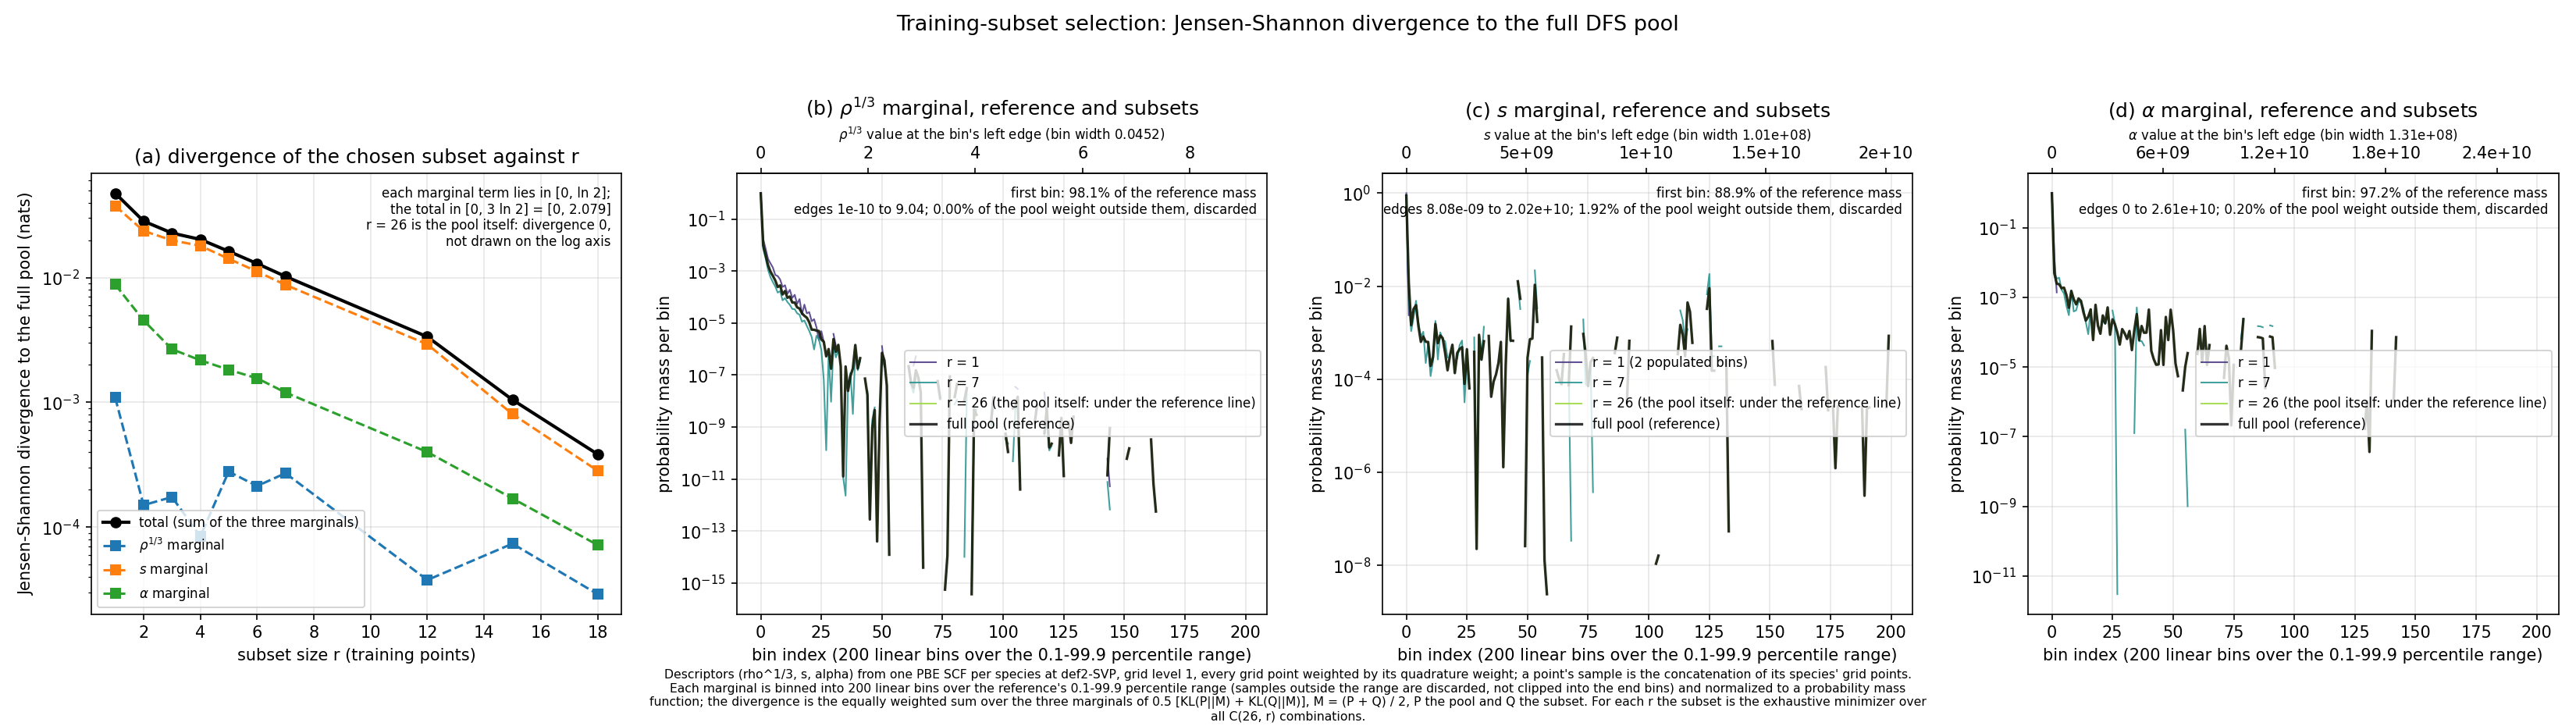
\includegraphics[width=0.72\linewidth]{figures_dfs_step7_v7_subsets/subset_jsd_vs_full.png}
  \end{center}
\end{frame}
\slidenote{The idea of the selection is to pick, for each subset size, the subset of training points whose electron densities look most like the whole pool in the variables a GGA or meta-GGA functional sees. Those variables are $\rho^{1/3}$ (the density, compressed), $s$ (the reduced gradient) and $\alpha$ (the iso-orbital indicator); they are computed once per species from a cheap PBE calculation on a small basis and a coarse grid, at every quadrature point of that species' grid. \textbf{Marginal:} the one-dimensional distribution of one of the three variables. \textbf{Histogram and mass function:} the range of each variable between its 0.1th and 99.9th percentile over the whole pool is cut into 200 equal bins; each grid point adds its quadrature weight to the bin its value falls in, and the histogram is normalized to sum to one, so that it is a probability mass function independent of the number of grid points or of the bin width. \textbf{The figure:} left, the divergence of the chosen subset from the pool against the subset size (total and the three marginal terms, log scale; the full pool has divergence zero and is not drawn on a log axis); right, the three reference mass functions (black) with the subsets at 1, 7 and 26 points overlaid, against the bin index, with the bin's variable value on the upper axis. The first bin dominates each marginal; the reasons are on the next slide.}

\begin{frame}{2. Subsets: the metric and the search [Lin91]}
  \small
  The distance between a candidate subset $S$ and the pool is the Jensen-Shannon divergence [code: subset\_selection.py:213--246, 472] summed over the three marginals with equal weights, $P_x$ the pool and $Q_x$ the subset mass function, probabilities floored at $10^{-12}$, natural logarithm:
  \[
  \mathrm{JSD}(S) = \sum_{x \in \{\rho^{1/3},\, s,\, \alpha\}} \tfrac12 \left[ \mathrm{KL}(P_x \,\|\, M_x) + \mathrm{KL}(Q_x \,\|\, M_x) \right], \qquad
  M_x = \tfrac12 (P_x + Q_x),
  \]
  \[
  \mathrm{KL}(P \,\|\, Q) = \sum_b P^{(b)} \ln \frac{P^{(b)}}{Q^{(b)}}, \qquad \text{each marginal term in } [0, \ln 2].
  \]
  For each $r \in \{1,\ldots,7, 12, 15, 18, 26\}$ the subset is the exhaustive minimizer over all $\binom{26}{r}$ combinations (9.7 million at $r = 12$); a subset with no grid point inside a marginal's range gets an infinite divergence.
  \begin{itemize}
    \item The linear edges reach the low-density tails ($s$ to $2.0\times10^{10}$, $\alpha$ to $2.6\times10^{10}$, $\rho^{1/3}$ from $10^{-10}$ to 9.04), so the first bin holds 98.1, 88.9 and 97.2 percent of the weighted reference mass: the whole chemical range for $s$ and $\alpha$, the vacuum tail ($\rho < 9.2\times10^{-5}$) for $\rho^{1/3}$.
    \item The metric therefore compares the low-density tails of the molecular grids ($s$, $\alpha$) and the valence and core region ($\rho^{1/3}$); the $s$ term is 74 to 89 percent of every divergence.
  \end{itemize}
\end{frame}
\slidenote{\textbf{Kullback-Leibler divergence} $\mathrm{KL}(P\|Q)$ measures how different a distribution $P$ is from $Q$; it is zero when they coincide and is not symmetric. \textbf{Jensen-Shannon divergence} is its symmetrized, bounded form: each distribution is compared with the average $M$ of the two, so it is symmetric and, with the natural logarithm, lies between 0 and $\ln 2$ per marginal; the three marginals are summed with equal weight, so the total lies between 0 and $3\ln 2 = 2.08$. "Natural logarithm" is what the report's "in nats" meant: a nat is the unit of information when logarithms are natural rather than base 2 (bits); the choice only scales the numbers. The $10^{-12}$ floor avoids $\ln 0$ in empty bins. \textbf{The search} is exhaustive: every subset of size $r$ is scored, using the fact that histograms add over disjoint samples so the per-point histograms are pre-binned once. \textbf{Why the first bin dominates:} the bin edges are linear over the 0.1 to 99.9 percentile range, and on a molecular quadrature grid the low-density tail carries enormous $s$ and $\alpha$ values (the density falls exponentially while its gradient and kinetic terms do not fall as fast), so the range stretches to $10^{10}$ and the whole chemically relevant range of $s$ and $\alpha$ ($s \lesssim 5$, $\alpha \lesssim 10$) falls in bin 0; for $\rho^{1/3}$ the opposite holds: bin 0 covers only $\rho < 9.2\times10^{-5}$ (vacuum), and the valence and core densities occupy the higher bins. The metric therefore compares subsets mainly on how their grids' low-density tails are distributed, which is a property of the selection as it was run and is stated rather than changed here because every trained cell used these subsets. The L2 alternative was computed and stored but no training run used it.}

\begin{frame}{2. Subsets: the chosen subsets [ledger subset\_index\_log.json; plot\_subset\_jsd.py]}
  \begin{center}\tiny\setlength{\tabcolsep}{2pt}
  \begin{tabular}{rp{7.6cm}lllll}
  \toprule
  $r$ & Points (ledger index order) & AE / BH76 / IP & JSD & $\rho^{1/3}$ & $s$ & $\alpha$ \\ \midrule
  1 & H2O & 1 / 0 / 0 & 0.0475 & 0.00109 & 0.03764 & 0.00881 \\
  2 & HLi, OH+N2\_to\_H+N2O & 1 / 1 / 0 & 0.0284 & 0.00015 & 0.02372 & 0.00455 \\
  3 & OH+N2\_to\_H+N2O, OH+CH3\_to\_O+CH4, Li\_IP & 0 / 2 / 1 & 0.0228 & 0.00017 & 0.01995 & 0.00267 \\
  4 & CH2, OH+N2\_to\_H+N2O, OH+CH3\_to\_O+CH4, Li\_IP & 1 / 2 / 1 & 0.0203 & 0.00008 & 0.01801 & 0.00218 \\
  5 & HLi, OH+N2\_to\_H+N2O, OH+CH3\_to\_O+CH4, Li\_IP, C\_IP & 1 / 2 / 2 & 0.0163 & 0.00028 & 0.01418 & 0.00183 \\
  6 & HLi, CH, OH+N2\_to\_H+N2O, OH+CH3\_to\_O+CH4, Li\_IP, C\_IP & 2 / 2 / 2 & 0.0130 & 0.00021 & 0.01120 & 0.00156 \\
  7 & CHN, CO2, HLi, CH, OH+N2\_to\_H+N2O, Li\_IP, C\_IP & 4 / 1 / 2 & 0.0102 & 0.00027 & 0.00877 & 0.00120 \\
  12 & CO2, C2H2, CO, HLi, CH, NO2, CH2, OH+N2\_to\_H+N2O, OH+CH3\_to\_O+CH4, HF+F\_to\_H+F2, Li\_IP, C\_IP & 7 / 3 / 2 & 0.0034 & 0.00004 & 0.00292 & 0.00040 \\
  15 & FLi, CHN, CO2, C2H2, CO, HLi, NO, CH, NO2, CH2, OH+N2\_to\_H+N2O, OH+CH3\_to\_O+CH4, HF+F\_to\_H+F2, Li\_IP, C\_IP & 10 / 3 / 2 & 0.0010 & 0.00007 & 0.00081 & 0.00017 \\
  18 & N2, FLi, CHN, CO2, C2H2, CO, HLi, Na2, NO, CH, NO2, N2O, CH2, OH+N2\_to\_H+N2O, OH+CH3\_to\_O+CH4, HF+F\_to\_H+F2, Li\_IP, C\_IP & 13 / 3 / 2 & 0.0004 & 0.00003 & 0.00028 & 0.00007 \\
  26 & the whole pool & 21 / 3 / 2 & 0 & 0 & 0 & 0 \\
  \bottomrule
  \end{tabular}
  \end{center}
  \scriptsize
  \begin{itemize}
    \item The $\rho^{1/3}$, $s$ and $\alpha$ columns are the three marginal terms of the JSD (their sum is the total); every value is recomputed from the descriptor caches and agrees with the ledger to $10^{-9}$. The subsets are nested only where the minimizer happens to nest; the 2-to-6-point subsets are barriers and ionizations with one or two molecules.
  \end{itemize}
\end{frame}
\slidenote{Each row is the training subset of one column of cells: the cells "at $r$ points" of every architecture were trained on exactly these points. \textbf{AE / BH76 / IP} counts how many of the points are atomization energies, barrier reactions and ionization potentials. The one-point subset is H2O alone; the two-point subset is the LiH atomization with the OH + N2 barrier; from three to six points the minimizer picks the two barriers and the Li ionization plus at most one or two molecules, because a barrier reaction contributes four or five species' grids and therefore covers more of the pool's descriptor distribution than a single molecule. From seven points on, atomization energies dominate. This composition matters for the held-out results: the 2-to-6-point cells contain almost no atomization energies and generalize worst (Sec. 5). \textbf{Ledger:} the file the selection wrote in June, holding for each size the chosen indices and the divergence; the table's values are recomputed from the cached descriptors by the figure script and agree with the ledger to $10^{-9}$, so the numbers shown are the ones the selection actually used.}

% =====================================================================
\section{3. Pre-training}

\begin{frame}{3. Pre-training: targets and objective}
  \small
  Each network is fitted pointwise [code: pretrain.py:261--341, pretrain\_data\_gen.py] to reproduce its parent (PBE on the GGA rung, SCAN on the meta-GGA) on the parent's own densities of the DFS pre-training inventory plus every atom of the BH76 and W4-11 pools (38 systems on the GGA rung, 36 on the meta-GGA; the certificate re-evaluates 39 and 38), with a synthetic $(r_s, s, \alpha)$ mesh [DFS21 SI] at 30 percent of the weight:
  \[
  t_x = F_x^{\rm parent} - 1 = \frac{\epsilon_x^{\rm parent}}{\epsilon_x^{\rm LDA}} - 1, \qquad
  t_c = F_c^{\rm parent} - 1 = \frac{\epsilon_c^{\rm parent}}{\epsilon_c^{\rm PW92}} - 1,
  \]
  the exchange rows posed per spin channel at the doubled density $(2 n_\sigma, 4\sigma_{\sigma\sigma})$ [OP79]. The objective is the integration-weighted pointwise residual plus a per-system energy term:
  \[
  \begin{aligned}
  \mathcal{L}_{\rm pre} = {} & \frac{\sum_i w_i\,(F_i^{\rm NN} - 1 - t_i)^2}{\sum_i w_i}
  + w_E\,\frac{1}{N_{\rm sys}}\sum_{s}\Big(\sum_{i\in s} w^{\rm grid}_i\, n_i\,\epsilon_i^{\rm LDA}\, F_i^{\rm NN} - E_{xc,s}^{\rm parent}\Big)^2, \\
  & w_i = |n_i\, \epsilon_i^{\rm LDA}|\, w_i^{\rm grid}, \qquad w_E = 0.1 .
  \end{aligned}
  \]
  \begin{itemize}
    \item The energy term is needed because the pointwise residual alone does not bound a system's energy.
    \item Adam, 20000 steps, learning rate $10^{-3}$ to $10^{-5}$ from the midpoint, clip 1.0, a 20 percent validation slice scored every 50 steps with patience 300 checks [cfg \texttt{pretrain:}].
  \end{itemize}
\end{frame}
\slidenote{Pre-training is not training on reference data: it fits the network so that it \textit{produces} the parent functional, PBE or SCAN, pointwise. The target at each grid point is the parent's enhancement factor minus one (so that a zero network output means "equal to the parent's LDA baseline"), evaluated with libxc on the parent's own self-consistent densities. The systems are the DFS pre-training inventory plus every atom that appears in the benchmark pools, so that the clone is accurate on the atoms the training and held-out reactions use. A synthetic mesh of $(r_s, s, \alpha)$ values, not tied to any molecule, is mixed in at 30 percent of the weight to regularize the fit in regions molecules sample sparsely. The residual is weighted by $|n\,\epsilon_x^{\rm LDA}|$ times the quadrature weight, i.e. by how much each point contributes to the energy. The energy term compares, for each system, the network's exchange-correlation energy with the parent's: an earlier round showed that a clone with the smallest pointwise error could still be tens of kcal/mol off on atomization energies, because small pointwise errors that do not cancel between a molecule and its atoms add up; the term with $w_E = 0.1$ removes that. \textbf{Adam} is the optimizer, 20000 steps with a learning rate decaying linearly from $10^{-3}$ to $10^{-5}$ over the second half; 20 percent of the grid rows are held out and scored every 50 steps, the best snapshot is kept, and the fit stops if 300 checks pass without improvement.}

\begin{frame}{3. Pre-training: the fidelity certificate}
  \small
  The saved networks are re-evaluated [code: cluster/fidelity.py, grid\_config.py:287--312] on every system at the production basis and grid and compared with the parent:
  \[
  \Delta E_{xc,s} = E_{xc,s}^{\rm NN} - E_{xc,s}^{\rm parent}, \qquad
  \Delta AE = \Delta E_{xc,{\rm mol}} - \sum_A \Delta E_{xc,A},
  \]
  \[
  \max_{\rm atoms} |\Delta E_{xc,A}| \le 1.0\ \text{mHa}, \qquad
  \mathrm{mean}_{\rm mol} |\Delta AE| \le 1.0\ \text{kcal/mol}, \qquad
  \max_{\rm mol} |\Delta AE| \le 2.0\ \text{kcal/mol}.
  \]
  A failing certificate holds the group's training array; every trained cell starts from a network that reproduces its parent to within these tolerances.
  \begin{center}\scriptsize
  \begin{tabular}{lllllll}
  \toprule
  Architecture & Parent & Loss X / C & max atom (mHa) & mean $|\Delta AE|$ & max $|\Delta AE|$ & Verdict \\ \midrule
  deep\_3x16 & PBE & 6.4e-8 / 7.6e-7 & 0.210 & 0.162 & 0.519 & PASS \\
  deep\_attn\_3x16 & PBE & 1.5e-8 / 6.7e-8 & 0.058 & 0.031 & 0.115 & PASS \\
  deep0\_3x16 & PBE & 2.8e-8 / 3.4e-6 & 0.439 & 0.114 & 0.450 & PASS \\
  deep0\_attn\_3x16 & PBE & 1.5e-8 / 9.9e-8 & 0.123 & 0.042 & 0.149 & PASS \\
  deep0\_cusp\_3x16 & PBE & 9.5e-8 / 1.1e-6 & 0.439 & 0.188 & 1.071 (AlCl3) & PASS \\
  deep0\_cusp\_mgga\_3x16 & SCAN & 3.7e-6 / 5.2e-6 & 3.132 & 2.062 & 7.257 (14 species) & FAIL \\
  \bottomrule
  \end{tabular}
  \end{center}
\end{frame}
\slidenote{The certificate is the proof that the pre-trained network is the parent functional for the purposes of the training that follows. It is computed at the production basis and grid (6-311++G(3df,2pd), grid level 3), not the pre-training grid, on the parent's frozen densities: for every system the difference of exchange-correlation energies between the clone and the parent, and for every molecule the resulting error in the atomization energy (the molecule's error minus its atoms' errors, since an atomization energy is a difference). The three tolerances are: no free atom more than 1 mHa off (0.63 kcal/mol), the mean atomization-energy error at most 1 kcal/mol, and no single molecule more than 2 kcal/mol off. The two-tier form (mean plus a worst-case backstop) replaced an earlier single 1 kcal/mol maximum, under which one species a few hundredths over the bound held an entire group while the set as a whole was far inside chemical accuracy. \textbf{Table columns:} the pointwise loss is the final value of the pre-training residual for the exchange (X) and correlation (C) networks; the species in parentheses are the molecules above 1 kcal/mol. Every GGA clone passes; the attention variants are the tightest clones. The one meta-GGA clone fails all three criteria; its exchange residual is 40 to 250 times the GGA clones' and its correlation residual 1.5 to 80 times, after the same number of steps, and its atomization errors (14 of 22 molecules above 1 kcal/mol, the eight largest of the same sign) mean the network does not reproduce SCAN well enough to serve as its starting point. The other four meta-GGA architectures' certificates are pending; until they exist the meta-GGA training array does not run.}

\begin{frame}{3. Pre-training: the loss curves}
  \begin{columns}[T]
  \begin{column}{0.5\linewidth}
    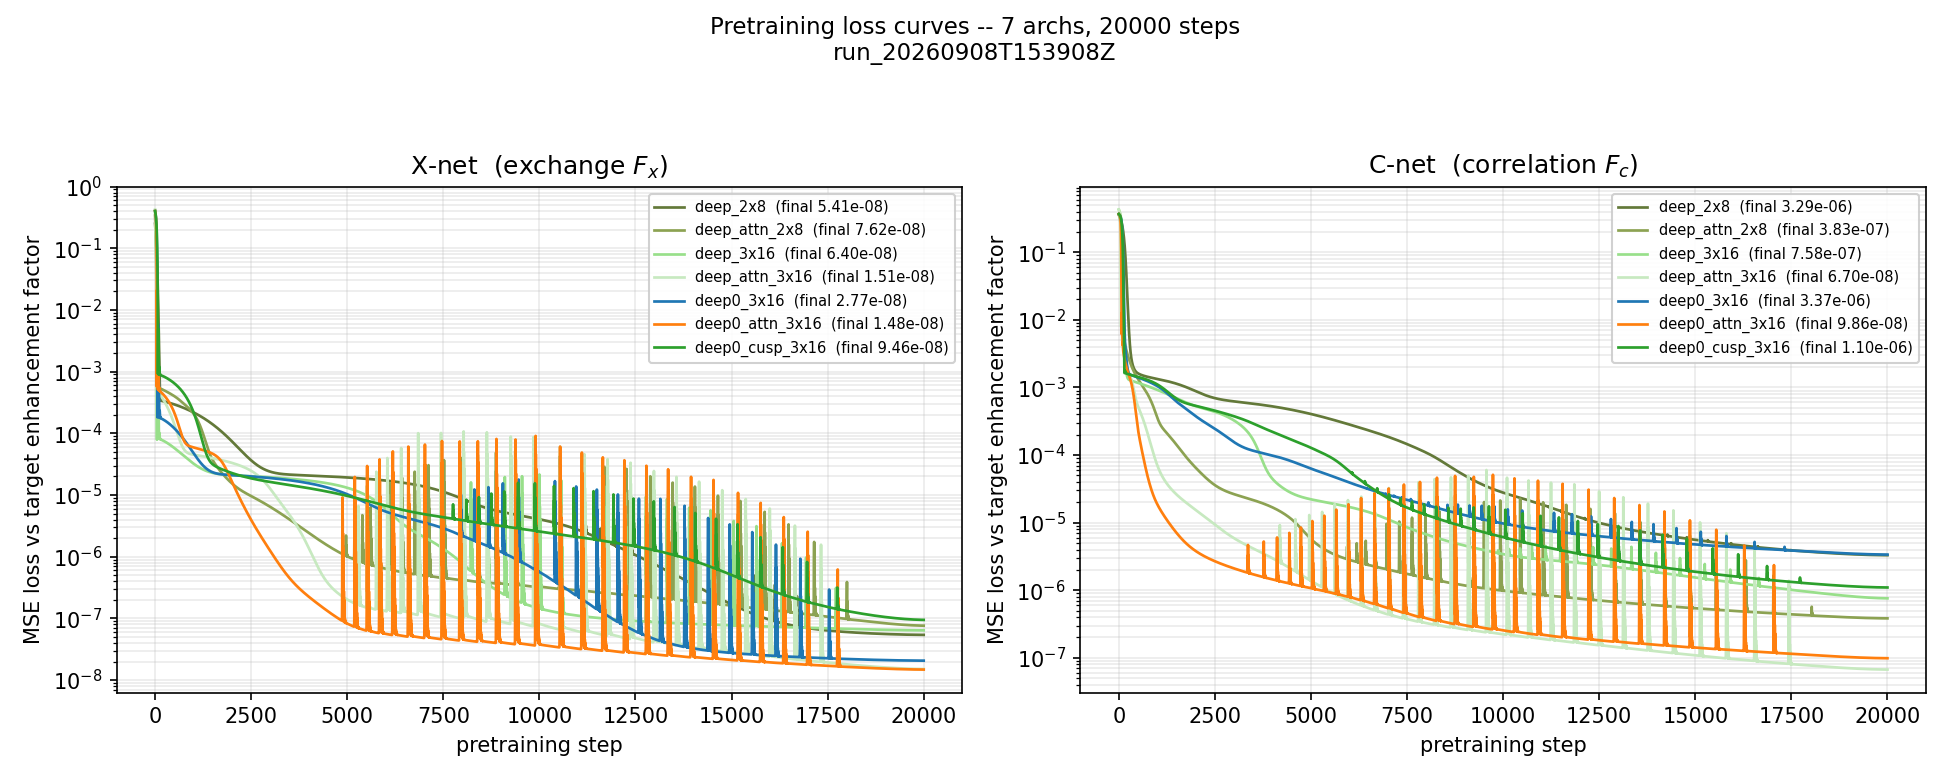
\includegraphics[width=\linewidth]{figures_dfs_step7_v7_family_pretrain/pretrain_curves.png}
  \end{column}
  \begin{column}{0.5\linewidth}
    
\includegraphics[width=\linewidth]{figures_dfs_step7_v7_family_pretrain/uncertified_mgga/pretrain_curves.png}
    \scriptsize
    \begin{itemize}
      \item Pointwise residual per step, exchange (left) and correlation (right); the spikes from step 5000 are the validation snapshot reloads.
      \item GGA clones end at $1.5\times10^{-8}$ to $9.5\times10^{-8}$ (exchange) and $6.7\times10^{-8}$ to $3.4\times10^{-6}$ (correlation); deep\_attn\_3x16 descends earliest and lowest, at the longest fit (28 h against 3.8 h for its plain twin).
      \item The SCAN clone (right) stops 40 to 250 times higher in exchange and 1.5 to 80 times in correlation after the same 20000 steps and fails the certificate (previous slide). Its four siblings are pending; the meta-GGA training array is held.
    \end{itemize}
  \end{column}
  \end{columns}
\end{frame}
\slidenote{Left: the seven certified GGA clones of the size and families runs on one panel pair; right: the meta-GGA clone (its certificate failed, so it is drawn from its run). The curves are the first term of the pre-training objective, the weighted mean squared pointwise residual, for the exchange network (left panel of each pair) and the correlation network (right panel), against the optimizer step on a log scale; the final value of each curve is in the legend. The regular spikes from step 5000 onward are an artifact of the validation procedure: every 50 steps the network is scored on the held-out rows and the best snapshot is reloaded, and the first step after a reload sits above the trend for one step. The GGA clones all reach residuals of order $10^{-8}$ to $10^{-6}$ in units of the squared enhancement-factor difference, which corresponds to sub-kcal/mol atomization errors (previous slide). The attention variants take much longer per step (28 h against 3.8 h) but reach the lowest residuals. The SCAN clone's curves are smooth and still decreasing slowly at 20000 steps; it does not diverge, it is simply far from converged to SCAN's accuracy, which is consistent with the meta-GGA form (an additional input, $x_\alpha$, and SCAN's more structured dependence on $\alpha$) needing more capacity or more steps than the GGA clones.}

\begin{frame}{3. Pre-training: the pre-trained networks against their parents}
  \begin{columns}[T]
  \begin{column}{0.5\linewidth}
    
\includegraphics[width=\linewidth]{figures_dfs_step7_v7_family_pretrain/pretrain_fx_fc_delta_all.png}
  \end{column}
  \begin{column}{0.5\linewidth}
    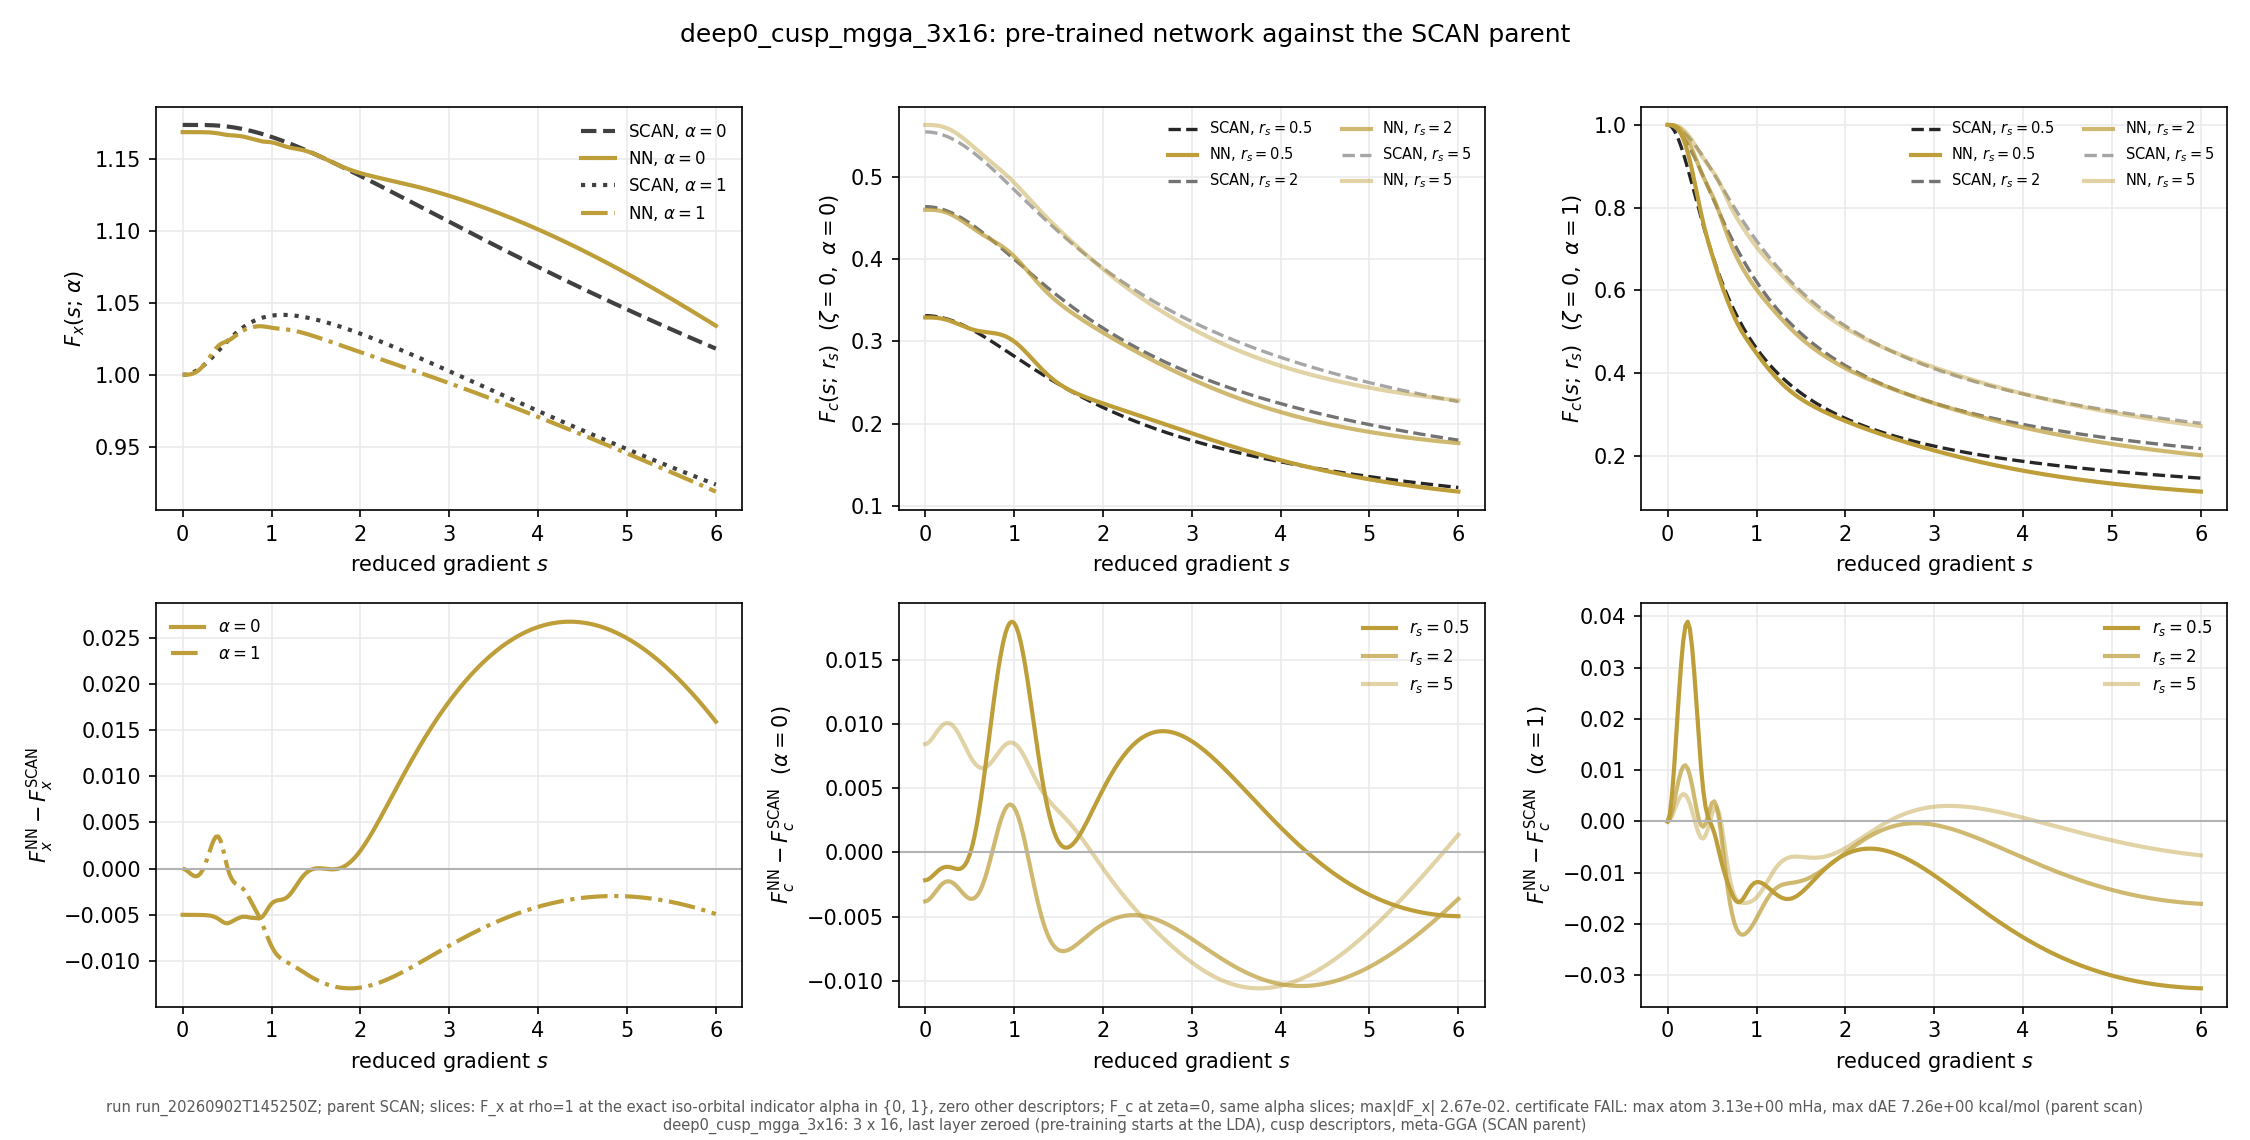
\includegraphics[width=\linewidth]{figures_dfs_step7_v7_family_pretrain/uncertified_mgga/pretrain_fx_fc_deep0_cusp_mgga_3x16.png}
    \scriptsize
    \begin{itemize}
      \item Left: the difference $F^{\rm NN} - F^{\rm PBE}$ of every GGA clone, exchange at $n = 1$ and correlation at $r_s = 2$, along $s$. Within $10^{-3}$ for $s < 2.5$, at most 0.007 at $s = 6$ (deep\_3x16 exchange); the three zero-init clones within $4.2\times10^{-3}$ everywhere.
      \item Right: the SCAN clone. $F_x(\alpha = 0)$ is 0.01 to 0.027 above SCAN for $s > 2.5$, $F_c(\alpha = 1)$ 0.0003 to 0.016 below it from $s = 2$ at $r_s = 2$ (0.005 to 0.033 at $r_s = 0.5$); same-sign offsets over wide $s$ ranges do not cancel between a molecule and its atoms.
    \end{itemize}
  \end{column}
  \end{columns}
\end{frame}
\slidenote{These figures show how closely each pre-trained network reproduces its parent along one-dimensional slices of the input space: the exchange enhancement factor as a function of $s$ at unit density, and the correlation factor as a function of $s$ at $r_s = 2$ (and, for the meta-GGA clone, at fixed $\alpha = 0$ and $\alpha = 1$, the two slices SCAN's paper uses). \textbf{The left figures} draw only the differences from PBE, one curve per architecture; the titles printed inside these PNGs read "pretrained corrections", a wording left from the plotting script, whereas the curves are the plain differences $F^{\rm NN} - F^{\rm PBE}$ of networks that were fitted to produce PBE, not to correct it (the correction to PBE is what the training of Sec. 4 produces). For $s$ below 2.5, where most of the energy-weighted grid points lie, every GGA clone is within $4 \times 10^{-3}$ of PBE (the four plain clones within $1.5 \times 10^{-3}$ in exchange); the differences grow beyond $s = 3$, a region the pre-training set samples sparsely, but stay below 0.007. \textbf{The right figure} is the meta-GGA clone against SCAN, with the parent dashed and the network solid and the difference panels beside them: the clone is above SCAN in exchange at $\alpha = 0$ over a wide range of $s$ and below it in correlation at $\alpha = 1$, and offsets of one sign over wide ranges are exactly what does not cancel in an atomization energy (molecule minus atoms), which is why this clone fails the certificate while its pointwise residual is 40 to 250 times the GGA clones' in exchange and 1.5 to 80 times in correlation.}

% =====================================================================
\section{4. Optimization, in-sample}

\begin{frame}{4. In-sample: the training objective [DFS21 Eqs. 15--17]}
  \small
  One optimizer step per training group per epoch (a reaction, or a molecule with its density and potential references); the group loss is the DFS weighting ($\lambda_{RE} = 1$, $\lambda_n = 20$), with $E^{\rm NN}$ the self-consistent energy of the $N = 3$ cycle SCF and $t$ the cycle:
  \[
  \mathcal{L} = 1\cdot\mathcal{L}_{AE} + 1\cdot\mathcal{L}_{\rm rxn} + 1\cdot\mathcal{L}_{IP} + 1\cdot\mathcal{L}_{v_{xc}} + 20\cdot\mathcal{L}_{\rho},
  \]
  \[
  \mathcal{L}_{\rm rxn} = \frac{1}{|T|}\sum_{t\in T} w_t^2\, r_t^2, \qquad
  r_t = \sum_i c_i\, E^{\rm NN}_{i,t} - E^{\rm ref}, \qquad
  w_t = \left(\frac{t}{N-1}\right)^2,
  \]
  \[
  \mathcal{L}_{AE} = 0.01\,\mathrm{mean}_Z\, \frac{(E_Z^{\rm NN} - E_Z^{\rm anchor})^2}{(E_Z^{\rm anchor})^2}, \qquad
  \mathcal{L}_{IP} = \mathrm{mean}\,(E^{\rm NN}_{+} - E^{\rm NN}_0 - IP^{\rm ref})^2, \qquad
  \mathcal{L}_{v_{xc}} = \frac{\|V_{xc}^{\rm NN} - V_{xc}^{\rm ref}\|_F^2}{n_{\rm AO}^2},
  \]
  \[
  \mathcal{L}_{\rho} = \mathrm{mean}_{\rm mol}\,\frac{\sum_g w_g\,(n^{\rm NN}_g - n^{\rm ref}_g)^2}{N_e^2}, \qquad N_e = \sum_g w_g\, n^{\rm ref}_g .
  \]
  \begin{itemize}
    \item $\mathcal{L}_{\rm rxn}$ is the DFS convergence-tail scoring ($w_t^2 = 0, 1/16, 1$ at $N = 3$) over the W4-11 atomizations, as reactions with the network's own atoms, and the BH76 barriers [W411, GMTKN55]; the free atoms are held near their exact energies [Chak93]; $V_{xc}$ is compared on the reference density; the density against CCSD on the same grid, per electron. Code: losses.py:76, 366--396; train.py:1829--1835; oneshot.py:632--653.
  \end{itemize}
\end{frame}
\slidenote{This is the actual training step, the only stage that changes the functional away from PBE. \textbf{Group and epoch:} the training data is organized in groups, each a reaction (with its reference energy) or a molecule (with its reference density and potential); one epoch takes one gradient step per group. \textbf{The five channels:} $\mathcal{L}_{\rm rxn}$, the reaction-energy residual: $r_t$ is the reaction energy formed from the network's self-consistent species energies at SCF cycle $t$ (with stoichiometric coefficients $c_i$) minus the reference, and the loss weights the last cycles most (at three cycles the weights are 0, 1/16 and 1), the DFS device that penalizes an SCF that does not settle instead of scoring one arbitrary cycle; the W4-11 atomization energies enter here as reactions "molecule to atoms" using the network's own atomic energies, beside the BH76 barrier heights. $\mathcal{L}_{AE}$, the atom anchors: the free atoms of the subset are held near their exact non-relativistic energies (Chakravorty et al.), as a relative error with the DFS weight 0.01, so that the absolute energy scale is not free to drift. $\mathcal{L}_{IP}$, ionization potentials (cation minus neutral against the reference). $\mathcal{L}_{v_{xc}}$, the exchange-correlation potential matrix compared with a reference potential obtained by inverting the reference density, on the reference density (this channel is not part of the DFS objective). $\mathcal{L}_\rho$, the density: the squared difference between the network's final SCF density and the CCSD reference density on the same grid, divided by the electron count squared so that molecules of different size weigh alike (DFS Eq. 17). The weights 1 and 20 are the Letter's $\lambda_{RE}$ and $\lambda_n$.}

\begin{frame}{4. In-sample: the training losses (deep\_3x16)}
  \begin{center}
  
\includegraphics[width=\linewidth,height=0.56\textheight,keepaspectratio]{figures_dfs_step7_v7_family_val_best/training_loss_channels_deep_3x16.png}
  \end{center}
  \scriptsize
  \begin{itemize}
    \item SCF: 3 cycles from the converged PBE density, DFS mixing $D_{t+1} = (1 - a_t) D_t + a_t D^{\rm out}_t$, $a_t = 0.3^{t} + 0.3$ [DFS21 SI], gradients through every cycle, the last mixed density scored. AdamW $10^{-3} \to 10^{-5}$ over the second half, weight decay $10^{-4}$, clip 1.0, 200 epochs, validation MAE on 35 reactions every 25 epochs.
    \item The reaction channel falls in every cell, by 3x (deep0\_3x16 at 18) to 190x (deep\_attn\_3x16 at 2); the density channel by 1.3x to 4.6x, both settled within 25 epochs. The potential channel, absent from the DFS objective, rises from 7 to 18 points in the plain networks (deep\_3x16 at 18: 3.9e-5 to 4.3e-5) and falls in deep\_attn\_3x16 at 12 and 15.
    \item Validation MAE: the 2-to-6-point cells of deep\_3x16 and deep0\_3x16 rise after the first check (deep\_3x16 at 2: 11.7 to 32.7 kcal/mol, best at epoch 25); the cells from seven points hold 6 to 11 kcal/mol; deep\_attn\_3x16's small cells fall (37 to 7 kcal/mol).
  \end{itemize}
\end{frame}
\slidenote{\textbf{The figure} has eight panels for the deep\_3x16 architecture, one curve per subset size (dark: one point, yellow: twenty-six), each a per-epoch mean on a log scale: the total loss, then the five channels at their trained weights (the five add up to the total), the validation reaction-energy error at each 25-epoch check with the chosen (validation-best) epoch starred, and the learning rate. \textbf{The SCF:} the network's energies and densities are self-consistent, but only three Kohn-Sham cycles are run from the converged PBE density, with the DFS linear mixing schedule (the new density is mixed into the old with a weight $a_t$ that decays from 1.3 toward 0.3); gradients flow through all three cycles. Three cycles are enough when the functional is close to PBE and do not converge when it is far from a fixed point, which is one of the reasons the held-out density comparison is asymmetric (Sec. 5); a 25-cycle variant is running. \textbf{AdamW} is the optimizer with decoupled weight decay; the learning rate is held for the first half of the run and decayed linearly over the second. \textbf{What the curves show:} the reaction channel is the one the training reduces by orders of magnitude; the density channel falls modestly and settles within 25 epochs; the potential channel rises for the larger subsets of the plain networks (and falls in the attention cells at 12 and 15), i.e. the potential term and the energy terms pull in different directions once many molecules are supervised. The validation error (reactions not in the training subset) separates the cells into two families: the cells trained on 2 to 6 points start overfitting after 25 epochs (their validation error rises), while the one-point cell and every cell from seven points holds 6 to 11 kcal/mol; the validation-best checkpoint is the epoch with the lowest validation error, so the small cells are read at epoch 25.}

\begin{frame}{4. In-sample: the trained enhancement factors}
  \begin{columns}[T]
  \begin{column}{0.5\linewidth}
    
\includegraphics[width=\linewidth]{figures_dfs_step7_v7_family_val_best/trained_fx_fc_deep_3x16.png}
  \end{column}
  \begin{column}{0.5\linewidth}
    
\includegraphics[width=\linewidth]{figures_dfs_step7_v7_family_val_best/trained_fx_fc_deep_attn_3x16.png}
  \end{column}
  \end{columns}
  \scriptsize
  \begin{itemize}
    \item Exchange, every architecture and subset: the trained $F_x$ is below PBE by 0.01 to 0.06 near $s = 0.8$ and above it from $s \approx 1.4$, by up to 0.18 (deep\_3x16), 0.13 (deep\_attn\_3x16), 0.14 (deep0\_3x16) at $s = 2.5$ to 3; the one-molecule cells of deep\_3x16 and deep0\_3x16 move least at $s = 0.8$.
    \item Correlation at $r_s = 2$: the one-molecule cells fall from 1 to 0.16 by $s = 2$ and to 0 beyond; the other cells stay between 0.45 and 1.3 up to $s = 2$ (PBE falls to 0.02 by $s = 3$), then split: deep\_3x16 at 2, 3, 5, 6, 15, 18, 26 decays to 0.1 to 0.6 by $s = 6$ while 4, 7 and 12 rise to 1.1 to 1.3; every deep\_attn\_3x16 cell but the one-molecule one rises above 1 (up to 1.9 at $s = 6$).
  \end{itemize}
\end{frame}
\slidenote{These are the trained functionals themselves, drawn along the same slices as the pre-training figures: the exchange factor against $s$ at unit density (top left of each figure), its difference from PBE (top right), the correlation factor at $r_s = 2$ (bottom left) and its difference (bottom right), one curve per subset size, at the validation-best checkpoint. Because every cell started from the PBE clone, each curve shows what the training on that subset changed. The exchange change has the same shape in every cell and architecture: a small reduction of $F_x$ at $s$ around 0.8 (the range of most valence density) and a raise between $s = 1.5$ and $s = 6$ (the density tails and the bonding regions), largest for the cells trained on few points. The correlation change is larger and varies more between cells: PBE's correlation enhancement decays quickly with $s$, while the trained networks keep it near 1 out to $s = 2$ and beyond that either decay slowly or rise above 1 depending on the cell, i.e. the training data at $r_s = 2$ and large $s$ does not determine the correlation factor. The differences from PBE are of order 0.1 to 1, not small perturbations, and the held-out section measures whether they transfer to reactions outside the training subset.}

\begin{frame}{4. In-sample: energy and density in DFS units on the training reactions}
  \begin{center}
  
\includegraphics[width=\linewidth,height=0.64\textheight,keepaspectratio]{figures_dfs_step7_v7_family_val_best/insample_by_pool_3x3_eps.png}
  \end{center}
  \scriptsize
  \begin{itemize}
    \item Rows WTMAD-2 / $\varepsilon_n$ / $\mathcal{ED}$ (Sec. 5 for the definitions), columns BH76 / W4-11 / combined; bars against PBE on each cell's own training reactions (caps), the dashed line PBE on their union (18.6, 3.83, 5.67 kcal/mol).
    \item All 33 cells are below PBE on $\mathcal{ED}$ over their own reactions: training WTMAD-2 0.00 to 4.4 kcal/mol against 5.67 on the union of the training reactions, deep\_attn\_3x16 0.05 to 2.45, deep0\_attn\_3x16 0.05 and 0.77. The grid-RMSE density of the trained molecules is below PBE in every cell (NN/PBE 0.72 to 0.97 deep\_3x16, 0.57 to 0.76 deep\_attn\_3x16, 0.68 to 0.93 deep0\_3x16); the per-electron $\varepsilon_n$ of deep\_3x16 is above the pooled PBE value from 2 to 18 points.
  \end{itemize}
\end{frame}
\slidenote{"In-sample" means measured on the very reactions and molecules the cell was trained on: this checks that the training reached what it was asked for, not whether it generalizes. \textbf{The nine panels} use the same layout and metrics as the held-out figure of Sec. 5 (defined there): the top row is the energy error (WTMAD-2), the middle row the density error per electron ($\varepsilon_n$), the bottom row their combination ($\mathcal{ED}$); the columns split the reactions into the BH76 barriers, the W4-11 atomizations, and both together. Each bar is one cell; the black cap over it is PBE on exactly the same reactions; a triangle marks a cell below its cap; the dashed line is PBE on the union of all training reactions of the run. Cells whose subset has no reaction of a column (the one-point cell has no barrier; the three-point subset has no atomization) have no bar there. \textbf{Reading:} every cell reproduces its own training reactions far better than PBE, and its training molecules' densities better than PBE in the grid-RMSE measure (the density loss it was trained on); the per-electron L1 measure $\varepsilon_n$ of the middle row weights the density differently and ranks some small-subset cells above PBE, so the two measures do not agree on the small cells, and both are reported. \textbf{A panel that is not shown:} the figure suite also produces an in-sample atomization-energy panel that subtracts the network's molecular energy from \textit{fixed, exact} atomic energies rather than from the network's own atoms; that panel measures the network's absolute-energy offset (30 to 110 kcal/mol here), not the trained quantity, and is excluded from every document until it is computed with the network's own atoms.}

% =====================================================================
\section{5. Optimization, hold-out}

\begin{frame}{5. Held-out: the set and the metrics [Goe17; DFS21 Eqs. 20, 21]}
  \small
  Test set: GMTKN55 BH76 barriers and W4-11 atomization energies, minus the 35-reaction validation slice, each cell's training reactions and four duplicate barriers: 58 BH76 and 120 W4-11 reactions, 189 species with CCSD densities. PBE is evaluated on each cell's own slice; the functionals with the same 3-cycle SCF they trained with, PBE's density converged.
  \[
  \mathrm{WTMAD\text{-}2} = \frac{56.84}{N}\sum_{i\in\{\rm BH76,\,W4\text{-}11\}} N_i\,\frac{\mathrm{MAD}_i}{\overline{|\Delta E_{\rm ref}|}_i}, \qquad
  \varepsilon_n = \frac{1}{N_e}\int |n - n^{\rm ref}|\, d^3r, \qquad N_e = \int n^{\rm ref}\, d^3r,
  \]
  \[
  \mathcal{ED} = \frac{2}{1/E + 1/(\gamma D)}, \qquad
  D_{\rm RMSE} = \sqrt{\sum_g w_g (n_g - n_g^{\rm ref})^2 \Big/ \sum_g w_g}.
  \]
  \begin{itemize}
    \item WTMAD-2 over the two present subsets; alone, a pool reads $56.84\,\mathrm{MAD}_i / \overline{|\Delta E_{\rm ref}|}_i$, a scaled relative error. $\gamma = 1084.87$ kcal/mol on $\varepsilon_n$ (DFS units) or $\gamma = E_{\rm PBE}/D_{\rm PBE}$ on the grid RMSE (self-calibrated).
    \item A cell beats PBE when its $\mathcal{ED}$ is below PBE's on the same slice. Pooled PBE: 8.92 kcal/mol WTMAD-2, $\varepsilon_n$ 0.00923.
    \item The harmonic mean is set by its smaller leg: with $\gamma\varepsilon_n \approx 10$ kcal/mol here, 1 kcal/mol of $E$ moves $\mathcal{ED}$ by 0.4 to 0.7, the whole density spread by at most 1.5..
  \end{itemize}
\end{frame}
\slidenote{\textbf{Held-out} means reactions and molecules the cell never trained on. The test set is the union of two standard benchmarks, the BH76 barrier heights and the W4-11 atomization energies (from the GMTKN55 collection), with three removals: 47 reactions set aside as the validation slice used only to pick the checkpoint, the cell's own training reactions, and four barriers that appear twice under permuted reactant names; what remains is the cell's "slice", and PBE is scored on the same slice so the comparison is like for like. \textbf{WTMAD-2} is GMTKN55's weighted total mean absolute deviation: each benchmark's mean absolute error is divided by that benchmark's mean absolute reference value (so barriers, around 19 kcal/mol, and atomization energies, around 350 kcal/mol, count as relative errors) and scaled by 56.84 kcal/mol, the mean absolute reference value over all of GMTKN55; here only two of GMTKN55's 55 benchmarks are present, so the figures say "2-subset". $\varepsilon_n$ is the DFS density error: the integrated absolute density difference from the CCSD reference density, per electron (Eq. 20 of the Letter); the grid RMSE is the alternative root-mean-square measure the older figures use. $\mathcal{ED}$ (Eq. 21) combines an energy error and a density error as a harmonic mean, with $\gamma$ converting the density error into kcal/mol: in "DFS units" $\gamma$ is the Letter's published slope 1084.87 and the density leg is $\varepsilon_n$; in "self-calibrated units" $\gamma$ is chosen so that PBE's two legs are equal and the density leg is the RMSE. A harmonic mean is dominated by its smaller term, and since every functional here has a density leg near 10 kcal/mol after $\gamma$, differences in $\mathcal{ED}$ come mostly from the energy leg. "Beats PBE" is defined as a lower $\mathcal{ED}$ than PBE on the same slice.}

\begin{frame}{5. Held-out: energy and density in DFS units (full set)}
  \begin{center}
  
\includegraphics[width=\linewidth,height=0.6\textheight,keepaspectratio]{figures_dfs_step7_v7_family_val_best/holdout_by_pool_3x3_eps.png}
  \end{center}
  \scriptsize
  \begin{itemize}
    \item Energy (combined WTMAD-2, PBE 8.92): deep\_3x16 7.92 at one point, 9.61 to 13.97 at two to six, 6.44 to 7.41 from seven to eighteen, 8.23 at twenty-six; deep\_attn\_3x16 5.94 to 8.26 over its nine cells, below PBE at every one; deep0\_3x16 5.90 to 8.52, below PBE at 1, 3, 4 and 7 to 26, above at 2, 5, 6; deep0\_attn\_3x16 8.11 at one point, 13.64 at two.
    \item Density ($\varepsilon_n$, PBE 0.00923): at or above PBE in every cell but deep\_attn\_3x16 at five points (0.00883) and deep0\_attn\_3x16 at one (0.00906), by 0.2 to 28 percent.
    \item $\mathcal{ED}$: deep\_3x16 and deep0\_3x16 below PBE at 1, 7, 12, 15, 18, 26 (the two starts agree at every size); deep\_attn\_3x16 at every cell (lowest 7.40 to 7.73 at 5 to 7 points against 9.32 to 9.49); deep0\_attn\_3x16 at one point.
  \end{itemize}
\end{frame}
\slidenote{The same nine-panel layout as the in-sample figure, now on the held-out slice: rows energy / density / combination, columns barriers / atomizations / both; the greens are deep\_3x16 and deep\_attn\_3x16, the blue deep0\_3x16, the orange deep0\_attn\_3x16; the dashed line is PBE on the pooled slice and the black cap PBE on each cell's own slice; a triangle marks a cell below its cap. \textbf{Energy:} deep\_3x16 beats PBE with one training point (H2O alone) and with seven or more, and loses with two to six; deep\_attn\_3x16 beats PBE at every one of its nine cells. The one-point result is not an accident of the metric: the cell trained on one molecule changes the functional least. The two-to-six-point cells are the ones whose subsets are barriers and ionizations with almost no atomization energies (Sec. 2), and they overfit (Sec. 4); which property of the subsets causes the loss is not established. \textbf{Density:} in the per-electron measure the trained functionals are at PBE's level or above it (worse) in every cell but one; the next slide shows that a fixed set of species accounts for the excess. \textbf{Combination:} because the density legs are all close to PBE's, the $\mathcal{ED}$ verdict follows the energy verdict: deep\_3x16 below PBE at 1, 7, 12, 15, 18 and 26 points, deep\_attn\_3x16 everywhere. The largest subsets (18, 26) do not improve on 7 to 15.}

\begin{frame}{5. Held-out: the full set beside the set without the recurring density tail}
  \begin{columns}[T]
  \begin{column}{0.5\linewidth}
    
\includegraphics[width=\linewidth]{figures_dfs_step7_v7_family_val_best/holdout_by_pool_3x3_eps.png}
  \end{column}
  \begin{column}{0.5\linewidth}
    
\includegraphics[width=\linewidth]{figures_dfs_step7_v7_family_val_best_excl_tail/holdout_by_pool_3x3_eps.png}
  \end{column}
  \end{columns}
  \scriptsize
  \begin{itemize}
    \item Left, the full set (the previous slide's figure); right, the same figure with the recurring density tail removed from the density leg.
    \item The density tail recurs: over the 33 cells, bn (the largest ratio in 32 of the 33 cells), rkt17, cloo, bn3pi, cn, h2, rkt06 and cs are above 1.5x PBE in at least half of the cells carrying them. Without them (right) the deep\_3x16 column from seven points is within 5 percent of PBE's $\varepsilon_n$, deep\_attn\_3x16 below it at 1, 2, 5, 6, 7, 12, 15, deep0\_3x16 at 15 and 26, deep0\_attn\_3x16 at 1; the $\mathcal{ED}$ verdicts change only for deep0\_3x16 at three points.
    \item The comparison is asymmetric by protocol (an unconverged network density against converged PBE); the converged-SCF re-evaluation in flight is the direct test.
  \end{itemize}
\end{frame}
\slidenote{\textbf{Left:} the full set, all four architectures on one axis (the previous slide's figure); deep0\_3x16's combined verdicts match deep\_3x16's at every size (the architecture slide). \textbf{The density tail:} when the per-species density errors are listed, the same handful of species has errors several times PBE's in almost every cell: BN and its $^3\Pi$ state, CN, CS, ClOO, the transition states of OH + Cl (rkt17) and H + CH4 (rkt06), and H2. "Recurring" is the rule that defines the list: a species whose error exceeds 1.5 times PBE's in at least half of the cells that contain it and in at least two. These are multireference or open-shell cases, for which a single-determinant CCSD reference density is itself least reliable, and they are the species whose three-cycle SCF from the PBE seed is farthest from converged (their first-cycle energy step is the largest), so their network density is the least settled. The list is selected by the trained functionals' own errors, so removing it is a diagnostic view, not a model-free one; a model-free list (from a CCSD T1 diagnostic) and a converged-SCF re-evaluation are the pending jobs that replace it. \textbf{Right:} the same cells with those eight species removed from the density leg (the energy leg is unchanged): the density errors of the deep\_3x16 cells from seven points move to within 5 percent of PBE's and several deep\_attn\_3x16 cells go below it, i.e. apart from the tail the trained densities are at PBE's level. \textbf{Asymmetric by protocol:} the network density comes from three SCF cycles that have not converged, while PBE's density is a fully converged calculation; a converged-SCF evaluation of the same networks is running and is the direct test of whether the tail is a property of the functionals or of the three-cycle evaluation.}

\begin{frame}{5. Held-out: per-cell results, combined leg, DFS units [holdout\_by\_pool\_3x3\_eps.csv]}
  \begin{center}\tiny\setlength{\tabcolsep}{2.2pt}
  \begin{tabular}{llrrrrrrr|llrrrrrrr}
  \toprule
  Arch & $r$ & E NN & E PBE & eps NN & eps PBE & ED NN & ED PBE & $\Delta$ED & Arch & $r$ & E NN & E PBE & eps NN & eps PBE & ED NN & ED PBE & $\Delta$ED \\ \midrule
  deep\_3x16 & 1 & 7.92 & 8.92 & 0.00951 & 0.00923 & 8.96 & 9.46 & \textbf{-0.50} & deep\_attn\_3x16 & 7 & 5.94 & 8.92 & 0.00963 & 0.00923 & 7.57 & 9.49 & \textbf{-1.91} \\
  deep\_3x16 & 2 & 9.61 & 8.92 & 0.01071 & 0.00923 & 10.52 & 9.44 & +1.08 & deep\_attn\_3x16 & 12 & 6.61 & 8.92 & 0.01019 & 0.00923 & 8.27 & 9.56 & \textbf{-1.29} \\
  deep\_3x16 & 3 & 10.67 & 8.92 & 0.01068 & 0.00923 & 11.11 & 9.32 & +1.79 & deep\_attn\_3x16 & 15 & 6.47 & 8.92 & 0.00956 & 0.00923 & 7.97 & 9.60 & \textbf{-1.63} \\
  deep\_3x16 & 4 & 11.06 & 8.92 & 0.01182 & 0.00923 & 11.88 & 9.34 & +2.53 & deep0\_3x16 & 1 & 8.18 & 8.92 & 0.00997 & 0.00923 & 9.32 & 9.46 & \textbf{-0.14} \\
  deep\_3x16 & 5 & 13.97 & 8.92 & 0.01113 & 0.00923 & 12.96 & 9.32 & +3.64 & deep0\_3x16 & 2 & 9.16 & 8.92 & 0.01143 & 0.00923 & 10.54 & 9.44 & +1.10 \\
  deep\_3x16 & 6 & 13.51 & 8.92 & 0.01091 & 0.00923 & 12.62 & 9.34 & +3.28 & deep0\_3x16 & 3 & 7.99 & 8.92 & 0.01062 & 0.00923 & 9.44 & 9.32 & +0.12 \\
  deep\_3x16 & 7 & 6.44 & 8.92 & 0.01017 & 0.00923 & 8.13 & 9.49 & \textbf{-1.35} & deep0\_3x16 & 4 & 8.06 & 8.92 & 0.01160 & 0.00923 & 9.83 & 9.34 & +0.48 \\
  deep\_3x16 & 12 & 7.41 & 8.92 & 0.01047 & 0.00923 & 8.97 & 9.56 & \textbf{-0.59} & deep0\_3x16 & 5 & 10.48 & 8.92 & 0.01099 & 0.00923 & 11.16 & 9.32 & +1.83 \\
  deep\_3x16 & 15 & 6.89 & 8.92 & 0.01004 & 0.00923 & 8.44 & 9.60 & \textbf{-1.16} & deep0\_3x16 & 6 & 10.40 & 8.92 & 0.01097 & 0.00923 & 11.10 & 9.34 & +1.76 \\
  deep\_3x16 & 18 & 6.74 & 8.92 & 0.00999 & 0.00923 & 8.31 & 9.62 & \textbf{-1.31} & deep0\_3x16 & 7 & 5.90 & 8.92 & 0.01051 & 0.00923 & 7.77 & 9.49 & \textbf{-1.72} \\
  deep\_3x16 & 26 & 8.23 & 8.92 & 0.00973 & 0.00923 & 9.25 & 9.80 & \textbf{-0.55} & deep0\_3x16 & 12 & 7.11 & 8.92 & 0.01058 & 0.00923 & 8.78 & 9.56 & \textbf{-0.78} \\
  deep\_attn\_3x16 & 1 & 8.26 & 8.92 & 0.00925 & 0.00923 & 9.06 & 9.46 & \textbf{-0.40} & deep0\_3x16 & 15 & 7.10 & 8.92 & 0.01013 & 0.00923 & 8.63 & 9.60 & \textbf{-0.97} \\
  deep\_attn\_3x16 & 2 & 7.87 & 8.92 & 0.00972 & 0.00923 & 9.01 & 9.44 & \textbf{-0.43} & deep0\_3x16 & 18 & 6.82 & 8.92 & 0.00996 & 0.00923 & 8.37 & 9.62 & \textbf{-1.26} \\
  deep\_attn\_3x16 & 3 & 7.22 & 8.92 & 0.00981 & 0.00923 & 8.60 & 9.32 & \textbf{-0.72} & deep0\_3x16 & 26 & 8.52 & 8.92 & 0.00961 & 0.00923 & 9.38 & 9.80 & \textbf{-0.42} \\
  deep\_attn\_3x16 & 4 & 6.09 & 8.92 & 0.01020 & 0.00923 & 7.85 & 9.34 & \textbf{-1.49} & deep0\_attn\_3x16 & 1 & 8.11 & 8.92 & 0.00906 & 0.00923 & 8.89 & 9.46 & \textbf{-0.57} \\
  deep\_attn\_3x16 & 5 & 6.03 & 8.92 & 0.00883 & 0.00923 & 7.40 & 9.32 & \textbf{-1.92} & deep0\_attn\_3x16 & 2 & 13.64 & 8.92 & 0.01168 & 0.00923 & 13.14 & 9.44 & +3.70 \\
  deep\_attn\_3x16 & 6 & 6.09 & 8.92 & 0.00973 & 0.00923 & 7.73 & 9.34 & \textbf{-1.61} & & & & & & & & & \\
  \bottomrule
  \end{tabular}
  \end{center}
  \scriptsize
  \begin{itemize}
    \item E in kcal/mol (2-subset WTMAD-2), eps per electron, ED under $\gamma = 1084.87$ kcal/mol; E PBE and eps PBE are the pooled values, ED PBE the cell-slice value. $\Delta$ED = ED NN $-$ ED PBE: \textbf{bold, negative} marks a cell below PBE (22 of 33).
    \item Verdicts within about 5 percent of PBE depend on the leg and the units: under the plain-MAE leg deep\_attn\_3x16 at 3, 5 and 6 flip; under self-calibrated grid-RMSE units deep\_attn\_3x16 at 2 and deep0\_3x16 at 3 flip (holdout\_ed\_combined.csv). The deep\_3x16 and deep0\_attn\_3x16 verdicts are the same under every choice.
  \end{itemize}
\end{frame}
\slidenote{One row per finished cell, the numbers behind the bar charts, read from the CSV the figure writes. \textbf{E NN / E PBE:} the combined 2-subset WTMAD-2 of the cell and of PBE (the pooled PBE value, the same in every row). \textbf{eps:} $\varepsilon_n$, the per-electron density error, for the cell and for PBE (pooled). \textbf{ED NN / ED PBE:} the combination for the cell and for PBE evaluated on that cell's own slice (which is why ED PBE varies from row to row while E PBE and eps PBE do not: the cell's training reactions are removed from its slice). \textbf{$\Delta$ED} is the new column, the cell's combination minus PBE's on the same slice; a negative value, set in bold, is a cell that beats PBE. Twenty-two of the 33 cells do: every deep\_attn\_3x16 cell, deep\_3x16 and deep0\_3x16 at 1 point and at 7 points and above. The deep\_3x16 and deep0\_3x16 rows have the same sign at every shared size, the replicate agreement noted on the architecture slide. \textbf{Second bullet:} the verdict of a cell whose $\Delta$ED is within a few tenths of zero can change when the energy leg is the plain mean absolute error instead of WTMAD-2, or when the density leg is the grid RMSE with a self-calibrated $\gamma$ instead of $\varepsilon_n$ with the DFS $\gamma$; the deep\_attn\_3x16 cells at 2, 3, 5 and 6 are such cases. The deep\_3x16 verdicts do not depend on those choices; deep0\_3x16 at 3 points is the one plain-network cell that does.}

% =====================================================================
\section{6. Pending}

\begin{frame}{6. Pending work}
  \small
  \begin{itemize}
    \item Cells still queued: deep\_attn\_3x16 at 18 and 26, deep0\_attn\_3x16 from 3 to 26, deep0\_cusp\_3x16 at every subset.
    \item Meta-GGA group: four certificates pending; the deep0\_cusp\_mgga\_3x16 FAIL holds the training array. The choice between dropping the architecture, refitting with more capacity or a higher energy-term weight, and an anchored form follows the four results.
    \item Converged-SCF re-evaluation of the 33 finished cells (DIIS at $10^{-8}$ Ha) and the CCSD T1 diagnostics for a model-free multireference list: two cluster jobs pending.
    \item Two training arms on the deep\_3x16 architecture at 7, 12, 15, 18 and 26 points: 25 SCF cycles with the current protocol (arm A) and the dpyscf-parity protocol (arm B: no convergence freeze, the executed first-mix index, the randomized atomic/PBE seed, Adam with the plateau schedule, the DFS L2 and channel weights). Submitted 2026-09-08, no results yet.
    \item The figure suite's in-sample atomization-energy panel stays out of the documents until it uses the network's own atoms (it now subtracts fixed exact atomic energies and reports the absolute-energy offset).
  \end{itemize}
\end{frame}
\slidenote{\textbf{Queued cells:} the remaining columns of the size and families runs are on the cluster, as are the two arms (whose cells will carry the tags [25 cycles] and [dpyscf parity] on the same axis); the figures and tables regenerate from the same suite as they land, by one entry per run in family\_runs.yaml. \textbf{Meta-GGA:} the failed SCAN clone blocks the whole group; the decision waits for the other four architectures' certificates, which tell whether the meta-GGA form as such, or that one architecture, is the problem. "Anchored form" means writing the network as SCAN plus a correction rather than the whole factor; it is listed as one of the options. \textbf{Converged-SCF re-evaluation:} the same trained networks evaluated with a fully converged self-consistent field (DIIS, energy converged to $10^{-8}$ Ha) instead of three cycles, which makes the density comparison with PBE symmetric. \textbf{T1 diagnostic:} a standard measure of multireference character from the CCSD amplitudes; a list of species selected by it, rather than by the trained functionals' errors, gives a model-free version of the tail-excluded view. \textbf{The two arms:} arm A keeps everything as is but runs 25 SCF cycles; arm B reproduces the DFS reference code's protocol in every setting the code can express (the density seed mixed with an atomic guess, the mixing schedule as executed, Adam with a plateau learning-rate schedule, the Letter's regularization and channel weights, no potential channel). Both target the deep\_3x16 architecture on the subsets that generalize. \textbf{The excluded panel:} see the in-sample notes; an atomization energy computed against fixed exact atomic energies measures where the network's absolute energy scale sits, which is not a trained quantity; the panel returns once it is computed against the network's own atoms.}

\begin{frame}{References and sources}
  \scriptsize
  \begin{itemize}
    \item [DFS21] S. Dick and M. Fernandez-Serra, Phys. Rev. B 104, L161109 (2021), with its Supplemental Material; reference code dpyscf.
    \item [PBE96] J. P. Perdew, K. Burke and M. Ernzerhof, Phys. Rev. Lett. 77, 3865 (1996). \quad [PW92] J. P. Perdew and Y. Wang, Phys. Rev. B 45, 13244 (1992).
    \item [SCAN15] J. Sun, A. Ruzsinszky and J. P. Perdew, Phys. Rev. Lett. 115, 036402 (2015). \quad [PRSB14] J. P. Perdew, A. Ruzsinszky, J. Sun and K. Burke, J. Chem. Phys. 140, 18A533 (2014).
    \item [OP79] G. L. Oliver and J. P. Perdew, Phys. Rev. A 20, 397 (1979). \quad [Kato57] T. Kato, Commun. Pure Appl. Math. 10, 151 (1957). \quad [Steiner63] E. Steiner, J. Chem. Phys. 39, 2365 (1963).
    \item [Vas17] A. Vaswani et al., NeurIPS 30 (2017). \quad [Xio20] R. Xiong et al., ICML (2020), arXiv:2002.04745.
    \item [Lin91] J. Lin, IEEE Trans. Inf. Theory 37, 145 (1991).
    \item [Goe17] L. Goerigk et al., Phys. Chem. Chem. Phys. 19, 32184 (2017) (GMTKN55, WTMAD-2, BH76RC). \quad [W411] A. Karton, S. Daon and J. M. L. Martin, Chem. Phys. Lett. 510, 165 (2011). \quad [HK12] R. Haunschild and W. Klopper, J. Chem. Phys. 136, 164102 (2012). \quad [Chak93] S. J. Chakravorty et al., Phys. Rev. A 47, 3649 (1993). \quad [NIST] NIST Chemistry WebBook ionization energies.
    \item [code] the repository: \path{xcquinox/alec/networks.py}, \path{descriptors.py}, \path{metagga.py}, \path{config.py}, \path{xcquinox/net.py}, \path{xcquinox/alec/subset_selection.py}, \path{dfs_pool.py}, \path{training_points.py}, \path{pretrain.py}, \path{cluster/fidelity.py}, \path{cluster/grid_config.py}, \path{losses.py}, \path{train.py}, \path{oneshot.py}, \path{solver.py}, \path{evaluation.py}, \path{notebooks/analysis/make_ablation_arch_figure.py}; the figures and CSVs under \path{notebooks/analysis/figures_dfs_step7_*}; [cfg] the run configurations \path{hpcjobs/configs/dfs_step7.dfs6311_grid3_v7*.yaml}.
  \end{itemize}
\end{frame}
\slidenote{The bracketed keys throughout the deck resolve here. Equations are cited to the paper that defines them and to the repository line that implements them; values are cited to the CSV or run file they are read from; protocol settings to the run configuration files. The file paths are relative to the repository root.}
